\documentclass{sig-alternate}
\usepackage{color}
\usepackage[colorinlistoftodos]{todonotes}

%%%%% Uncomment the following line and comment out the previous one
%%%%% to remove all comments
%%%%% NOTE: comments still occupy a line even if invisible;
%%%%% Don't write them as a separate paragraph
%\newcommand{\mycomment}[1]{}

\begin{document}

% --- Author Metadata ---
\conferenceinfo{UMM CSci Senior Seminar Conference, November 2018}{Morris, MN}

\title{Software Development Practices in Startups}

\numberofauthors{1}

\author{
\alignauthor
John D. Hoff\\
	\affaddr{Division of Science and Mathematics}\\
	\affaddr{University of Minnesota, Morris}\\
	\affaddr{Morris, Minnesota, USA 56267}\\
	\email{hoffx247@morris.umn.edu}
}

\maketitle
\begin{abstract}
Abstract goes here.

\end{abstract}

\keywords{Startup, Agile, Lean, Requirements, Software Development}

\section{Introduction}
\label{sec:introduction}
What is a startup? What are some challenges faced by startups?

\section{Background}
\label{sec:background}

\subsection{Methodologies}
\label{sec:methodologies}
Agile and lean.

\subsection{Requirements Practices}
\label{sec:practices}
While there are numerous practices in software development, this paper focuses on six that most closely relate to requirements gathering in software startups: requirements artefacts, knowledge management, requirements-related roles, planning, technical debt, and product quality. Requirements gathering is the process of documenting tasks that need to be completed to continue product development. These are based on input from customers, developers, and product owners. 

\section{The Evolution of Requirements Practices}
\label{sec:practicesEvolution}
Using Grounded Theory, the evolution of software development practices was studied at 16 software startups by Catarina Gralha et. al. They define these startups as "organizations in search of a scalable, repeatable, profitable business model or a human institution designed to create a new product or service under conditions of extreme uncertainty."~\cite{Gralha:2018} The goal of the study was to classify every practice of each software startup into one of three phases of evolution.


\subsection{Research Methods}
\label{sec:researchMethods}
To understand the evolution of requirements practices, two questions were asked at 16 software startups: how do requirements practices change, and what factors and turning points drive those changes?~\cite{Gralha:2018} These questions were used to learn about company growth, requirements gathering, requirements prioritization, features and knowledge management, and tools. The goal of this study is to determine which of the three phases of the six dimensions that each startup is currently at. Data was collected by conducting interviews, all-day observations, and attending project meetings. 

\subsection{Phases of Evolution}
\label{sec:reqPracticeEvolution}
Each dimension is "characterized by 3 phases of evolution."~\cite{Gralha:2018} The first phase is the beginning phase, where practices are unstructured. In the second phase, practices are semi-structured. In the third and final phase, practices are formally structured.  Every advance from one phase to the next is caused by at least one of eight turning points: number of clients, input from clients, negative feedback, retention rate of clients, revenue, number of employees, number of remote workers or flexible work hours, and number of features or products.~\cite{Gralha:2018} Phases of evolution for each specific dimension will be explained.

\subsubsection{Requirements Artefacts}
In the first phase, startups begin with little or no user input, making requirements artefacts implementation-orientated. The founders' backgrounds and company culture determine what tasks need to be done. Tasks are informally documented, sometimes on sticky notes. The second phase is user oriented. Startups look at feedback and input from their users to develop new tasks, known as user stories that are commonly documented with project management tools such as Confluence and Jira.~\cite{Gralha:2018} In the final phase, ``requirements artefacts evolve into richer, traceable descriptions."~\cite{Gralha:2018} Tasks are broken down into smaller, simpler tasks that are given effort-based estimations for time of completion. Tasks are formally prioritized, assigned to developers, and organized into products or releases.

\subsubsection{Knowledge Management}
Knowledge management is informal and unstructured in its first phase. Founders and developers rely on each other to complete tasks and manage the few features of their product. As the amount of tasks, features, and employees grow, startups enter the second phase where knowledge management is informal and semi-structured. Knowledge is shared through regular team and company meetings. Online communication tools, such as Slack, are used in place of ad hoc verbal communication. When a startup grows to a size that separates employees into different departments, knowledge management is formally structured. Using tools such as Slack and GitHub, communication and project management are often intertwined.

\subsubsection{Requirements-Related Roles}
Startups begin with general and multiple requirements-related roles where ``everyone does everything." Once a startup has clients, they move to the second phase where roles are semi-specific. Clients receive more attention and marketing staff are brought on, giving developers more room to focus on product development. In the final phase, roles are specific and single. Startups might decide to hire product managers and quality assurance specialists.

\subsubsection{Planning}
Startups do not have any planning in the first phase. Most time and resources are spent developing a working product that looks attractive to the market. Once a startup understands client needs, it moves to the second phase where planning is monthly and quarterly-oriented. Planning is based on client requests without deadlines. In the third phase, planning is strategic and aligned with vision. Companies prioritize features for a broader market and decide what is better for their clients.

\subsubsection{Technical Debt}
Technical debt is known and accepted in the earliest phase. As products become more complex, startups will track and record technical debt in the second phase. Hiring additional developers provides more resources to address some, but not all of a startup's technical debt. In the final phase, technical debt is managed and controlled. Tasks are specifically created to address this debt and prioritized with their associated features.

\subsubsection{Product Quality}
In the first phase, "speed of release takes precedence over quality."~\cite{Gralha:2018} With minimal testing, there are higher rates of negative feedback due to defective features. To avoid negative feedback, startups move to the second phase where product quality is somewhat important. User experience and scalability become critical. Product quality eventually becomes a top priority in the last phase due to its correlation with company reputation.

\begin{figure}
\centering
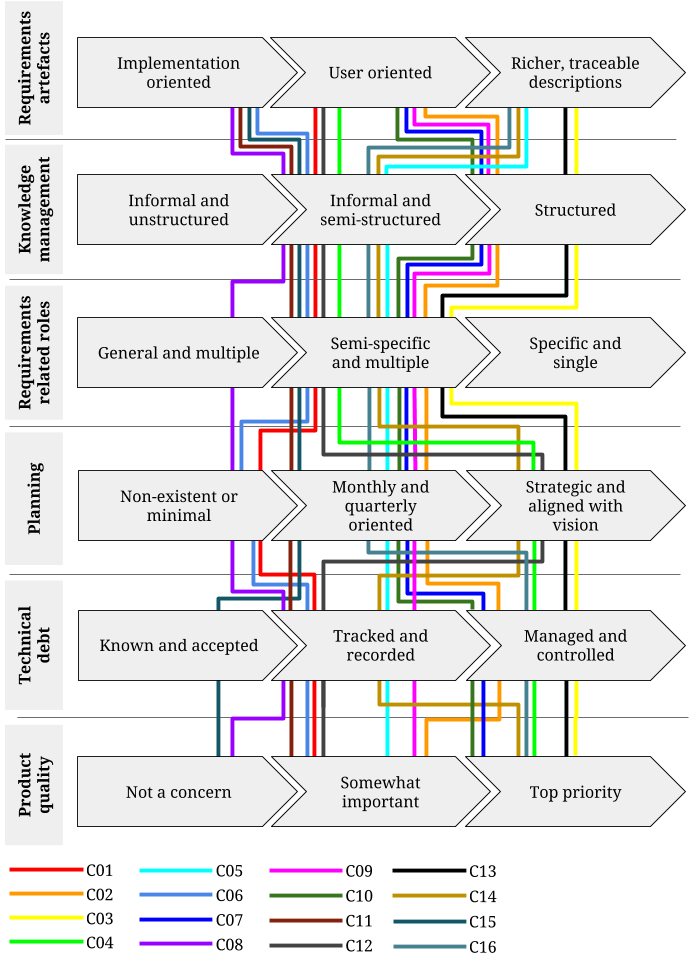
\psfig{file=companies-dimensions.png,width =3.4in}
\caption{Companies' Phases of Evolution}
\label{fig:companiesEvolution}
\end{figure}

\subsection{Discussion}
\label{sec:discussion}
In a fast-paced and reactive environment, startups ignore the long run in order to capture a market, retain clients, and release products quicker. Evolution along the six dimensions are not fundamental to success. Factors that cause startups to die can be a combination of the market of its product, human resources, culture, funding, processes, and practices.

Figure~\ref{fig:companiesEvolution} shows which phase of evolution of the six dimensions that each of the 16 companies are currently at. No startup reached the third phase of requirements-related roles and all had left the first phase of knowledge management. Company C06, a 10 year-old startup is only at phase one or two in every dimension.  It was reported that the work environment at C06 was stressful and had long hours. C03, one of the furthest along every dimension, was a 4 year-old startup with 11-20 employees. These contrasting profiles indicate that movement along the three phases of evolution is not dependent on company age and size. 



\section{Conclusions}
\label{sec:conclusions}

\section*{Acknowledgments}
\label{sec:acknowledgments}

Thanks Elena and Nic!

% The following two commands are all you need in the
% initial runs of your .tex file to
% produce the bibliography for the citations in your paper.
\bibliographystyle{abbrv}
% sample_paper.bib is the name of the BibTex file containing the
% bibliography entries. Note that you *don't* include the .bib ending here.
\bibliography{sample_paper}  
% You must have a proper ".bib" file
%  and remember to run:
% latex bibtex latex latex
% to resolve all references

\end{document}
